\chapter{Аналитическая часть}

В данном разделе представлено теоретическое описание КРМ-схемы хранения разреженных матриц и алгоритмов обработки матриц.

\section{КРМ-схема хранения разреженных матриц}

Для начала следует описать схему хранения разреженной матрицы, предложенную Кнутом. Ненулевые элементы хранятся в компактной форме в одномерном массиве $AN$. Информация о положении ненулевых элементов в матрице хранится двумя дополнительными параллельными одномерными массивами --- $I$ и $J$; здесь для каждого ненулевого элемента содержатся его строчный и столбцовый индексы. Итак, для каждого $a_{ij} \neq 0$ в памяти находится тройка $(a_{ij}, i, j)$. Далее, чтобы можно было легко отыскивать элементы произвольной строки или столбца матрицы, необходимы еще пара указателей для каждой тройки, а также указатели входа для строк и столбцов, сообщающие начало каждого строчного или столбцового списка. Пусть NR («next nonzero element in the same row» --- «следующий ненулевой элемент той же строки») --- массив, хранящий строчные указатели, а NC («next nonzero element in the same column» --- «следующий ненулевой элемент того же столбца») --- массив столбцовых указателей.
Пять массивов AN, I, J, NR и NC имеют одинаковую длину, и их одноименные позиции соответствуют друг другу. Пусть JR и JC --- массивы, содержащие указатели входа для строк и столбцов, расположенные в соответствии с порядком строк и столбцов матрицы. Тогда рассмотрим матрицу на рис. \ref{img:matrix}, её представление с помощью схемы Кнута --- на рис. \ref{img:knuth}.

\begin{figure}[H]
	\begin{center}
		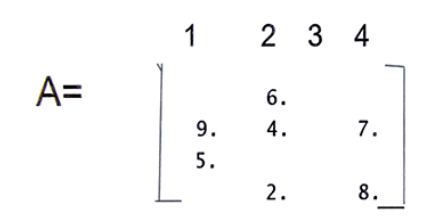
\includegraphics[scale=0.7]{img/matrix.png}
	\end{center}
	\captionsetup{justification=centering}
	\caption{Разреженная матрица}
	\label{img:matrix}
\end{figure}

\begin{figure}[H]
	\begin{center}
		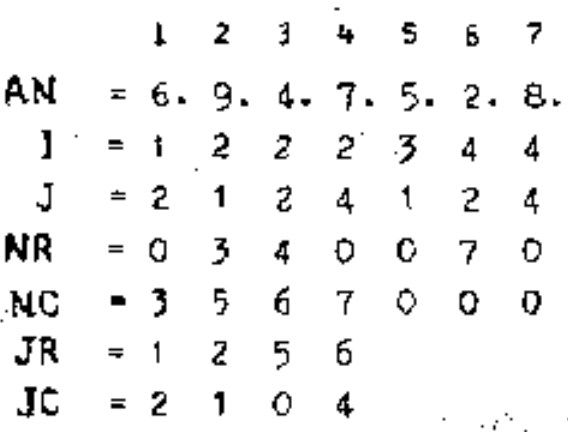
\includegraphics[scale=0.7]{img/knuth.png}
	\end{center}
	\captionsetup{justification=centering}
	\caption{Схема Кнута}
	\label{img:knuth}
\end{figure}

Рейнболдт и Местеньи предложили модификацию схемы Кнута, сохраняющую ее ценные свойства, но использующую значительно меньше накладных расходов по памяти. Она получила название схемы Кнута-Рейнбол-дта-Местеньи, или кольцевая КРМ-схема. Связные списки строк и столбцов закольцовываются, а начальные позиции списков включаются в указатели входа. Списки, ассоциированные со строками (столбцами), попарно не пересекаются и потому могут быть совместно хранимы одним массивом NR (для столбцов --- NC). Для матрицы на рис. \ref{img:matrix} \cite{tads} приведено ее представление с помощью КРМ-схемы на рис. \ref{img:krm}. Эта схема более плотная по сравнению со схемой Кнута. Однако, если приходится просматривать элементы некоторой строки (или столбца), то в сжатом формате нет никакой информации о столбцовых (строчных) индексах этих элементов~\cite{krm}.

\begin{figure}[H]
	\begin{center}
		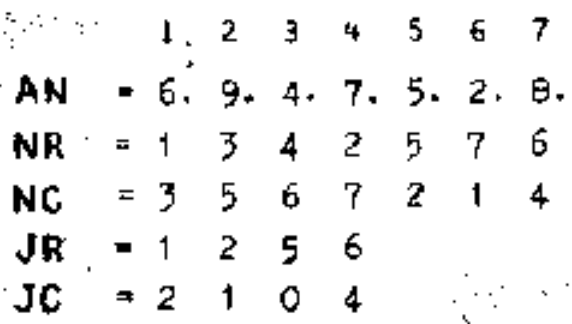
\includegraphics[scale=0.7]{img/krm.png}
	\end{center}
	\captionsetup{justification=centering}
	\caption{Кольцевая КРМ-схема}
	\label{img:krm}
\end{figure}

\section{Последовательный алгоритм}

В некоторых задачах происходит обработка матриц перед
их использованием в решении. Данные проходят ряд преобразований в
несколько последовательных этапов. Каждый этап реализуется при помощи алгоритма работы с матрицами.

В данной лабораторной работе будет реализована обработка разреженных матриц, состоящая из следующих этапов:
\begin{itemize}
	\item генерация упакованной верхнетреугольной матрицы в КРМ-схему хранения;
	\item удаление элементов из матрицы, меньших, либо равных $q$ ($q$ - задано);
	\item вывод исходной и измененной матрицы в файл.
\end{itemize}

\section{Алгоритмы, выполняемые на отдельных лентах}

Каждый из описанных выше этапов будет выполняться на отдельной ленте.

\subsection{Генерация верхнетреугольной упакованной в КРМ-схему хранения матрицы}

Генерация верхнетреугольной упакованной в КРМ-схему хранения матрицы будет происходить следующим образом:
\begin{enumerate}
	\item Значение каждого элемента матрицы, стоящего над главной диагональю и на ней, рандомно генерируется и записывается в массив $AN$.
	\item Если это не последний элемент в строке, то в массив $NR$ записывается (номер текущего элемента + 1).
	\item Если сгенерированный элемент --- последний элемент в строке, то в массив $NR$ записывается (номер текущего элемента + номер текущей строки --- номер текущего столбца).
	\item Если элемент находится не на главной диагонали, то в массив $NC$ записывается (номер текущего элемента + размерность матрицы $-$~номер текущей строки).
	\item Если элемент находится на главной диагонали, то в массив $NC$ записывается (номер текущего элемента $-$ размерность матрицы $\cdot$ номер текущей строки + (1 + номер текущей строки) $\cdot$ номер текущей строки / 2) и в массив $JR$ записывается номер текущего элемента.
	\item Если элемент находится на первой строке, то в массив $JC$ записывается номер текущего элемента.
\end{enumerate}


\subsection{Удаление из матрицы элементов, меньших либо равных $q$}

Для получения из верхнетреугольной матрицы набора матриц, из которых исключены значения, меньшие или равные $q$, где $q$ --- заданное значение, необходимо в цикле по ненулевым элементам матрицы на каждой итерации удалить элемент, если он меньшие или равен $q$. Для удаления элемента из матрицы нужно удалить его из массива $AN$, хранящего значения ненулевых элементов. Затем в массивах $NR$ и $NC$ изменить следующее: тот, кто ссылался на удаляемый элемент, теперь должен ссылаться на элемент, на который ссылался удаляемый. Значения номеров элементов, большие удаляемого, в массивах $NR$ и $NC$ должны уменьшиться на 1. В массивах $JR$ и $JC$ в случае, когда удаляется последний элемент в строке (столбце) записать 0 в позицию массива $JR$ ($JC$), равную номеру строки. В остальных случаях, когда удаляемый элемент является первым в строке (столбце) и в этой строке (столбце) есть другие элементы, надо вместо номера удаляемого элемента в массив $JR$ ($JC$) записать номер элемента, на который ссылается удаляемый элемент в массиве $NR$ ($NC$). Значения номеров элементов, большие удаляемого, в массивах $JR$ и $JC$ также должны уменьшиться на 1.

\subsection{Вывод матрицы в файл}

Вывод матрицы в файл будет происходить в следующем порядке.
\begin{enumerate}
	\item Вывод массива $AN$.
	\item Вывод массива $NR$.
	\item Вывод массива $NC$.
	\item Вывод массива $JR$.
	\item Вывод массива $JC$.
\end{enumerate}

\section{Параллельный алгоритм}

При помощи многопоточности можно ускорить процесс обработки матриц.
В этом случае для каждой ленты создается отдельный поток. Извлечение
и добавление матриц осуществляется потоками. Так, в параллельном алгоритме работа распределяется следующим образом:
\begin{itemize}
	\item первый поток извлекает матрицу из первой очереди, она обрабатывается на первой ленте, и поток добавляет ее во вторую очередь;
	\item второй поток извлекает матрицу из второй очереди, она обрабатывается на второй ленте, и поток добавляет ее в третью очередь;
	\item третий поток извлекает матрицу из второй очереди, и она обрабатывается на третьей ленте;
	\item каждый поток по завершении вновь извлекает матрицу из своей очереди, и цикл обработки повторяется в параллельном режиме.
\end{itemize}

\section*{Вывод}

В данном разделе были описаны основные положения КРМ-схемы хранения разреженных матриц, последовательный и конвейерный алгоритмы обработки матриц.